\documentclass[
12pt,draftcls,onecolumn%
%journal
%9pt,technote
]{IEEEtran}
%\usepackage{epstopdf}
%\epstopdfsetup{suffix={}}

\usepackage{graphicx}  % Written by David Carlisle and Sebastian Rahtz
\usepackage{subfigure}  % Written by Steven Douglas Cochran
\graphicspath{
{figs/matlab/}
{figs/ipe/}
{figs/img/}
}


\usepackage{amssymb}    % added by w.g.
\usepackage{amsmath,bm}    % From the American Mathematical Society
\usepackage{amsthm}
\usepackage{mathrsfs}

\usepackage{hyperref}

%%%%\usepackage[width=11cm,font=footnotesize,labelfont=bf, %
%%%%format=default,justification=centerlast]{caption} % Figure caption text customization 
%%%\usepackage{hyperref}
\usepackage[colorinlistoftodos]{todonotes} %side notes and comments
%%%
\usepackage{siunitx} % for units like degree, ...
\sisetup{unitsep=\cdot} % for commands like \SI{50}{\ohm} etc.

%%%\DeclareMathOperator*{\smargmin}{arg\,min}
%%%\DeclareMathOperator*{\smargmax}{arg\,max}
%%%
\newtheorem{theorem}{Theorem}
\newtheorem{assumption}{Assumption}
\newtheorem{lemma}{Lemma}
\newtheorem{proposition}{Proposition}
\newtheorem{remark}{Remark}
\newtheorem{corollary}{Corollary}
%%%% correct bad hyphenation here
%%%\hyphenation{op-tical net-works semi-conduc-tor}

\begin{document}
%
% paper title
% can use linebreaks \\ within to get better formatting as desired
%\title{Time Varying Operator for Controlling Nonholonomic Systems with Drift}
\title{Universal Control Law for Nonholonomic Systems with Drift}

\author{Md Suruz~Miah,~\IEEEmembership{Senior Member,~IEEE}% and 
%		N.~U.~Ahmed                
\thanks{S.~Miah is with the Electrical and Computer Engineering Department, Bradley University, Peoria, IL, 61625, USA. e-Mails:~smiah@bradley.edu}% <-this % stops a space
%\thanks{S.~Miah is with the Electrical and Computer Engineering Department, Bradley University, Peoria, IL, 61625, USA. e-Mail:~smiah@bradley.edu}% <-this % stops a space

%\thanks{N.~Ahmed is with the School of Electrical Engineering and Computer Science, University of Ottawa, Ottawa, ON, K1N 6N5, CANADA. e-Mail:~\{ahmed\}@eecs.uottawa.ca}% <-this % stops a space


\thanks{This research supported in part by Caterpillar Inc.}
}
% The paper headers
%\markboth{Journal of \LaTeX\ Class Files,~Vol.~6, No.~1, January~2007}%

% make the title area
\maketitle

\begin{abstract}
A universal control law for nonholonomic systems with drift is considered. While the development of feedback control laws for controlling nonlinear dynamical systems are well-established in the literature to date, the need of a control theoretic method to establish a universal control law for a class of nonlinear systems is significant. 
This is simply because the formulation of feedback control laws  relies on types of dynamical systems to be controlled which lead to a significant technical challenge for researchers.% to propose a general feedback law for a class of  nonlinear dynamical systems. %This task is even more challenging when the system is only partially observable. 
%
Here we underscore the need for a universal control law  that is aimed to address the trajectory tracking problem of nonholonomic systems with drift. For that, we propose to develop a time-varying feedback operator (called  herein a universal control law), to solve the tracking problem. The objective of the current manuscript is to prove the existence and to establish necessary conditions of the proposed time-varying feedback operator for nonholonomic systems with drift. The performance of the time-varying feedback operator will be backed up by a set of computer simulations. The novelty of this research lies in the modularity of the control law despite inherent non-linearity of nonholonoic systems. 
%
%complex dynamical systems.%, such as differential drive mobile robots, underwater or flying vehicles, and  competitive systems (\textit{e.g.,} mixing of renewable and nonrenewable energy sources). 

\end{abstract}

% Note that keywords are not normally used for peerreview papers.
\begin{IEEEkeywords}
Generalized control law, nonholonomic systems, drift, Pontryagin's minimum principle.
\end{IEEEkeywords}
\IEEEpeerreviewmaketitle

%%%%%%%%%%%%%%%%%%%%%%
\section{Introduction}

\section{Notations and Preliminaries}\label{sec:notations}
Throughout this paper, scalar and vector quantities will be denoted by non-bold letters and lower-case bold letters, respectively. Upper-case bold letters will denote matrices. For any positive integer $n$, $\mathbb{R}^n$ denotes the Euclidean space. For any vector ${\bf x,y}\in\mathbb{R}^n$, the standard Euclidean norm and the scalar product are given by
\begin{equation*}
\|{\bf x}\| \equiv  \left[\sum_{i=1}^n \left |x_i\right |^2\right]^{1/2}~\hbox{and}~~ {\bf (x\cdot y)}\equiv{\bf x}^T{\bf y}\equiv\sum_{i=1}^n x_i y_i, 
\end{equation*}
respectively. We shall use $\mathbb{R}^{m\times n}$ to denote the space of $m\times n$ matrices with entries from $\mathbb{R}$.  Let ${\bf X,Y}\in\mathbb{R}^{m\times n}$, then the standard norm and their scalar product are also given by 
\begin{equation*}
\begin{split}
\|{\bf X}\|\equiv\left[\sum_{i=1}^m \sum_{j=1}^n\left |x_{i,j}\right |^2\right]^{1/2}~\text{and}~{\bf (X\cdot Y)}\equiv Tr\left[{\bf X}^T{\bf Y}\right]\equiv Tr\left[{\bf X}{\bf Y}^T\right],
\end{split}
\end{equation*}
respectively, where $\mathrm{Tr}\left[\cdot\right]$ denotes the trace of matrix $\left[\cdot\right]$. Clearly, $\mathrm{Tr}\left[{\bf X}^T{\bf X}\right]=\|{\bf X}\|^2$. ${\bf X}\otimes {\bf Y}$ is the Kronecker product of two matrices ${\bf X,Y},$ where $\mathbb{R}^{m^2\times n^2}\ni {\bf Z} = {\bf X}\otimes {\bf Y}.$ $C({\cal I}, \mathbb{R}^n)$ is the class of all continuous function on the time interval ${\cal I}$ taking values from~$\mathbb{R}^n.$

If the function $J:\mathbb{R}^n\to \mathbb{R}$ is differentiable at ${\bf x}\in \mathbb{R}^n$, then for any ${\bf v}\in\mathbb{R}^n$, $dJ({\bf x};{\bf v})$ denotes the Gateaux (directional) derivative in the direction of ${\bf v}$, which is given by
%
\begin{equation*}
dJ({\bf x};{\bf v}) = {\bf v}^T\nabla J=\lim_{\varepsilon\to 0} \frac{J({\bf x} + \varepsilon{\bf v}) - J({\bf x})}{\varepsilon}, 
\end{equation*}
where $\nabla J$ denotes the gradient of $J$.
%
However, if $J:\mathbb{R}^{m\times n}\to \mathbb{R}$, then for any ${\bf X},{\bf V}\in\mathbb{R}^{m\times n}$, the directional derivative in the direction of ${\bf V}$ is defined by
\begin{equation*}
dJ({\bf X};{\bf V}) = Tr[{\bf V}^T\nabla J] = \lim_{\varepsilon\to 0} \frac{J({\bf X} + \varepsilon{\bf V}) - J({\bf X})}{\varepsilon}. 
\end{equation*}
For any bounded time interval ${\cal I} \equiv [0, t_f],~t_f>0,$ $C({\cal I},\mathbb{R}^n)$ denotes the class of all continuous functions on ${\cal I}$ taking values in $\mathbb{R}^n$. Let $p \in [1,\infty)$ and  any finite time interval ${\cal I}$, we use  ${\cal L}_p({\cal I},\mathbb{R}^n)$ to denote the set of Lebesgue measurable functions $\{{\bf f}\}$ defined on ${\cal I}$ and taking values in $\mathbb{R}^n$ whose norms are $p$-th power integrable,~\textit{i.e.,}~
%\begin{equation*}
$L_p({\bf f}) = \left(\int_{0}^{t_f}\|{\bf f}\|^p \mathrm{dt}\right)^{1/p}<\infty,$ 
%\end{equation*}
%
where $L_p({\bf f})$ denotes the $p$th norm of the function ${\bf f}$~\cite{Royden2010,Khalil2002}. For $p=\infty$, ${\cal L}_{\infty}({\cal I},R^n)$ denotes the space  of Lebesgue measurable functions $\{{\bf f}\}$ defined on ${\cal I}$ and taking values in $\mathbb{R}^n$ satisfying 
%
%\begin{equation*}
$\text{ess sup} \{ \|{\bf f}(t)\|, t \in {\cal I}\} < \infty.$
%\end{equation*}
%
% Similarly, ${\cal L}_p^{\ell oc}([0,\infty),\mathbb{R}^n)$ are locally convex topological vector spaces of $p$-th power locally integrable functions containing the  spaces ${\cal L}_p(I,\mathbb{R}^n)$.
%We use $\mathrm{diag}(a_1,\ldots,a_n)$ to represent a matrix whose diagonal entries starting in the upper left corner are $a_1,\ldots,a_n$.

\section{System Model and Problem Statement}
\label{sec:systemModel}
\subsection{System Model}
We consider a class of dynamical systems described by 
\begin{subequations}
\label{eq:system}
\begin{align}
\label{eq:systemModel}
\dot{{\bf q}}(t) & = \bar{{\bf g}}({\bf q}(t)) + \sum_{j=1}^m{\bf g}_j({\bf q}(t))u_j(t),\\
\label{eq:controlLaw}
u_j(t) & = {\bf k}_j^T(t) {\bf q}(t), 
\end{align}
\end{subequations}
where ${\bf q}(t)\in{\cal Q}\subset\mathbb{R}^n$ is the state of the system at time $t\ge 0$ with ${\cal Q}$ being its state space, $u_j$ is the $j$th, $j=1,\ldots, m$ control variable, and ${\bf k}_j: \mathbb{R}\to \mathbb{R}^n$ is the time-varying feedback operator of the $j$th control variable for positive integer $n,$ $m$ with $n>m$. The drift vector field $\bar{{\bf g}}:\mathbb{R}^n\to\mathbb{R}^n$ represents natural unforced motion of the system and ${\bf g}_j:\mathbb{R}^n\to\mathbb{R}^n,$ $j=1,\ldots,m,$ are linearly independent control vector fields~\cite{Choset2004}. When no ambiguity arises, we shall drop the argument $(t)$ for clarity. System~\eqref{eq:system} can also be written in compact form as
%
\begin{subequations}
\label{eq:system1}
\begin{align}
\label{eq:systemModel1}
\dot{{\bf q}} & = \bar{{\bf g}}({\bf q}) + {\bf G}({\bf q}){\bf u},\\
\label{eq:controlLaw1}
{\bf u} & = {\bf K}(t) {\bf q}, 
\end{align}
\end{subequations}
%
where ${\bf u}\in{\cal U}\subset \mathbb{R}^m$ is the vector of $m$ control inputs to the system, ${\bf G}:\mathbb{R}^n\to\mathbb{R}^{n\times m},$ and the time varying feedback operator ${\bf K}:\mathbb{R}_0^+\to{\cal K}_{\mathrm{ad}}\subset\mathbb{R}^{m\times n}.$ 


Note the difference in the feedback control law in~\eqref{eq:controlLaw1} with other existing control laws in the literature. It is simply a matter of determining the universal matrix (herein called feedback operator) ${\bf K}(t)\in{\cal K}\subset\mathbb{R}^{m\times n}.$  

\subsection{Problem Formulation} 
Let ${\bf q}^d(t)$ be the desired (reference) trajectory that the system~\eqref{eq:systemModel1} is supposed to track and $e(t) = \|{\bf q}(t)-{\bf q}^d(t)\|_{\mathbb{R}^n}$ denotes its state tracking error, for $t\in {\cal I}$. The objective is to find the optimal time-varying feedback operator  ${\bf K}(t)\in {\cal K}_{ad}$ that generates the trajectory ${\bf q}(t)\in{\cal Q}$ while minimizing the average cumulative state tracking error, $\mathscr{E}_{\mathrm{avg}}$, given by 
\begin{equation}
\mathscr{E}_{\mathrm{avg}} = \frac{1}{t_f}\int_{0}^{t_f}e(t)\mathrm{dt},~~t_f>0.
\label{eq:tracking-error}
\end{equation}

Given the system model~\eqref{eq:system1}, the problem can be stated as follows:
\begin{equation}
\inf_{\{{\bf q}\in{\cal Q},~{\bf K}\in{\cal K}_{ad}\}} [\mathscr{E}_{\mathrm{avg}}].
\label{eq:problem}
\end{equation}

\section{Proposed Universal Control Law}
\label{sec:feedbackOperator}
This section details the design procedure of the proposed universal time-varying control law, which is the main contribution of this manuscript. Substituting~\eqref{eq:controlLaw1} in~\eqref{eq:systemModel1}, yields the following full-state feedback system:
\begin{equation}
\begin{split}
\dot{{\bf q}}  = \bar{{\bf g}}({\bf q}) + {\bf G}({\bf q}){\bf K}(t) {\bf q} \equiv{\bf f}({\bf q},{\bf K}),
\end{split}
\label{eq:systemFeedbackFull}
\end{equation}
with ${\bf q}(0)={\bf q}_0.$ We emphasize that the generalized linear time varying operator ${\bf K}(t)$ completely characterizes the feedback law~\eqref{eq:systemFeedbackFull} for solving the trajectory tracking problem. 

\begin{lemma}[Solutions of feedback system]
\label{lem:feedback-sol}
Given the feedback system~\eqref{eq:systemFeedbackFull}, which is defined over the finite time horizon of ${\cal I}$, then for every initial condition ${\bf q}(0)\in\mathbb{R}^n$, and feedback operator ${\bf K}(t)\in {\cal K}_{ad}$, the system~\eqref{eq:systemFeedbackFull} has a unique absolutely continuous solution ${\bf q}(t)\in C({\cal I}, \mathbb{R}^n)$. Furthermore, the solution set ${\cal Q}\equiv\left\{{\bf q}(t) \equiv{\bf q}[t,{\bf K}(t)]\in C({\cal I},\mathbb{R}^n):{\bf K}(t)\in {\cal K}_{ad}\right \}$ is a bounded subset of $C({\cal I}, \mathbb{R}^n)$. 
\end{lemma}
%\begin{IEEEproof}
The proof of this lemma is classical and follows from a similar technique in~\cite[page~89]{Ahmed2006}. %
%\end{IEEEproof}
Hence, the actual trajectory of the of the vehicle can then be symbolically represented by 
\begin{equation}
{\bf q}(t) = {\bf q}(0) + \int_{0}^{t}{\bf f}[{\bf q}(\tau),{\bf K}(\tau)]d\tau,
\label{eq:actual-trajectory-full} 
\end{equation}
for $t\in {\cal I}$. In order to solve the trajectory tracking problem of nonholonomic systems with drift, let us introduce the cost functional as
\begin{equation}
J({\bf K}) = \Phi [t_f,{\bf q}(t_f)] + \int_{0}^{t_f} \ell [t,{\bf q}(t,{\bf K})]\mathrm{dt},~~\mathrm{with}
\label{eq:cost-fn}
\end{equation}
\begin{multline*}
\Phi [t_f,{\bf q}(t_f)]= \frac{1}{2} [{\bf q}(t_f)-{\bf q}^d(t_f)]^T{\bf P}(t_f)[{\bf q}(t_f)-{\bf q}^d(t_f)] ~\mathrm{and}~\\
\ell [t,{\bf q}(t)] =\frac{1}{2}[{\bf q}(t)-{\bf q}^d(t)]^T{\bf Q}(t)[{\bf q}(t)-{\bf q}^d(t)],
%\label{eq:cost-fn}
\end{multline*}
where the weight matrix ${\bf P}(t_f) \in\mathbb{R}^{n\times n}$ and the  tracking weight ${\bf Q}(t)\in\mathbb{R}^{n\times n}$ are symmetric positive definite matrices that indicate the relative importance of the error components along $\mathbb{R}^n.$ %
%
%If the vehicle's purpose is to stabilize on a fixed configuration, then ${\bf P}(t_f)$ must be higher than ${\bf Q}(t)$ and the desired trajectory is set to a \emph{fixed} configuration. However, the opposite is true for the vehicle to track a desired trajectory. 
%
The performance index $J({\bf K})$ in~\eqref{eq:cost-fn} depends on the feedback operator ${\bf K}(t)$ through the state variable ${\bf q}(t)$ as it is clear from the feedback system~\eqref{eq:systemFeedbackFull}. Note that $\Phi[\cdot]$ and $\ell[\cdot]$ of~\eqref{eq:cost-fn} are referred to as the terminal and tracking cost functionals, respectively. The task now becomes solving the following problem:
\begin{equation}
\inf_{{\bf K}\in{\cal K}_{ad}} [J({\bf K})],
\label{eq:problem1}
\end{equation}
which yields ${\bf q}(t) \to {\bf q}^d(t)$ as $J({\bf K})\longrightarrow 0$, for $t\in {\cal I}$. It is important to point out that, solving the problem~\eqref{eq:problem1} will eventually solve  the problem~\eqref{eq:problem}. Hence, the problem~\eqref{eq:problem1} can be solved if there exists a generalized optimal feedback operator ${\bf K}^*(t)$, for $t\in {\cal I}.$ However, it is worth noting the following remark before we proceed determining the generalized control law ${\bf K}(t).$ 
%

\begin{remark}
Note that the optimal feedback gain ${\bf K}(t)$ can be determined by following the classical Pontryagin's minimum principle~\cite[Chaper~8]{Ahmed2006} with ${\bf K}(t)$ being the open--loop control input to the feedback system~\eqref{eq:systemFeedbackFull}. For that, let $\mathrm{vec}({\bf K}(t))$ transforms the matrix ${\bf K}(t)$ into a column vector, which is formed by stacking the rows of ${\bf K}(t).$ The feedback model~\eqref{eq:systemFeedbackFull} can be rewritten as 
\begin{equation}
  {\bf \dot q} = \bar{{\bf g}}({\bf q}) + \left({\bf q}^T\otimes{\bf G}({\bf q})\right){\bf \bar k},
  \label{eq:systemFeedbackFull1}  
\end{equation}
where $\mathbb{R}^{nm}\ni{\bf \bar k}=\mathrm{vec}({\bf K})$ is now the control input vector that can be solved by following the standard gradient descent technique presented in~\cite[Chapter~3]{Stengel1994}~\cite[Chaper~8]{Ahmed2006}. By rearranging the elements of the optimal vector ${\bf \bar k}^*,$ we can reconstruct the optimal feedback operator ${\bf K}^*$ which is then substituted in the feedback law~\eqref{eq:systemFeedbackFull} to generate the optimal control input vector ${\bf u}^*(t),$ for $t\in{\cal I}.$  Nevertheless,  we emphasize in determining the optimal feedback operator ${\bf K}^*(t)$ directly by modifying the classical Pontryagin's minimum principle, which has applications in solving problems of a general class of partially observed dynamic systems. 
\end{remark}


\subsection{Existence of Generalized Control Law}
In this section, we provide the proof of the existence of the proposed generalized time-varying control law, ${\bf K}(t),$ that essentially solves the tracking problems of nonholonomic systems with drift. 

\begin{theorem}\label{thm:existence-K}
Given a nonholonomic system modeled by \eqref{eq:systemModel1}, there exists a generalized optimal control law ${\bf K}^*(t) \in {\cal K}_{ad}$ for the controller modeled in~\eqref{eq:controlLaw1} that drives the system~\eqref{eq:systemModel1} to the desired trajectory ${\bf q}^d(t)$ while finding the optimal solution for the problem~\eqref{eq:problem}. 
\end{theorem}
%%See Appendix~\ref{app:thm:existence-K} for its complete proof. %
 \begin{proof} 
Following the well known Alaoglu's theorem\footnote{\href{https://en.wikipedia.org/wiki/Banach/wiki/Banach–Alaoglu_theorem}{https://en.wikipedia.org/wiki/Banach/wiki/Banach–Alaoglu\_theorem}},  ${\cal K}_{ad} \subset {\cal K}\subset\mathbb{R}^{m\times n}$  is a (weak star) $w^*$ compact set and it suffices to prove that ${\bf K} \longmapsto J({\bf K})$ is sequentially weak star continuous. Let $\{{\bf K}^i, i \in \mathbb{N}\} \in {\cal K}_{ad}$ be a sequence  and suppose   ${\bf K}^i \buildrel w^* \over \to {\bf K}^*.$ Since ${\cal K}_{ad}$ is $w^*$ closed,  we have ${\bf K}^* \in {\cal K}_{ad}$, see~\cite{AhMi2011-j1}. 

Suppressing the variable $t$ for clarity, let $\{{\bf q}^i,~i\in \mathbb{N}\}$ and ${\bf q}^*$ denote the  solutions of the system~\eqref{eq:systemFeedbackFull} corresponding to $\{{\bf K}^i,~i\in \mathbb{N}\}$ and ${\bf K}^*$, respectively. Hence, the corresponding state equation becomes 
\begin{align*}
{\bf \dot q}^i = {\bf f}({\bf q}^i,{\bf K}^i)~\text{and}~
{\bf \dot q}^* = {\bf f}({\bf q}^*,{\bf K}^*),~{\bf q}^i_0={\bf q}^*_0={\bf q}_0.
\end{align*}
%
Using~\eqref{eq:actual-trajectory-full}, the solutions of the above two state-space models can be described by
\begin{equation*}
\begin{split}
{\bf q}^i(t) = {\bf q}_0 + \int_{0}^{t}{\bf f}[{\bf q}^i(\tau),{\bf K}^i(\tau)]d\tau,~\text{and}~~
{\bf q}^*(t)= {\bf q}_0 + \int_{0}^{t}{\bf f}[{\bf q}^*(\tau),{\bf K}^*(\tau)]d\tau.
\end{split}
\end{equation*}
%
Subtracting one from another, we get
\begin{align}
{\bf q}^i(t)-{\bf q}^*(t) = \int_{0}^t\left({\bf f}[{\bf q}^i(\tau),{\bf K}^i(\tau)]- {\bf f}[{\bf q}^*(\tau),{\bf K}^*(\tau)]\right)d\tau.
\label{eq:existence-temp1}
\end{align}
Note that ${\bf G}({\bf q}^i),~i\in \mathbb{N}$ and ${\bf G}({\bf q}^*)$ are uniformly bounded functions and satisfy Lipschitz condition
\begin{align*}
\|{\bf G}({\bf q}^i)-{\bf G}({\bf q}^*)\|&\leq L_{c2}\|{\bf q}^i-{\bf q}^*\|,\\
\|\bar{{\bf g}}({\bf q}^i)-\bar{{\bf g}}({\bf q}^*)\|&\leq L_{c1}\|{\bf q}^i-{\bf q}^*\|,\\
\end{align*}
where $L_{c1}$ and $L_{c2}$ are Lipschitz constants. Taking the Euclidean norm in both sides of expression~\eqref{eq:existence-temp1} and using the triangle inequality yield
\begin{align*}
\|{\bf q}^i(t)-{\bf q}^*(t)\| \leq v^i(t)+\int_{0}^t\beta(\tau)\|{\bf q}^i(\tau)-{\bf q}^*(\tau)\|d\tau,~\text{where}
\end{align*}
%
\begin{equation*}
v^i(t) = \Big\Vert\int_{0}^t\left[{\bf G}({\bf q}^i)({\bf K}^i-{\bf K}^*){\bf q}^i\right]d\tau\Big\Vert,
\end{equation*}
${\beta}(t) = (L_{c1} + c_1(t) + c_2(t)L_{c2}) \in{\cal L}_1^{+}({\cal I})$, with 
\begin{align*}
c_1(t)=[\sup \|{\bf G}({\bf q}^i)\|][\sup \|{\bf K}\|],~c_2(t) = \sup(\|{\bf K}^*\|\|{\bf q}\|),
\end{align*}
for $i\in \mathbb{N},~{\bf K}\in{\cal K},~\text{and}~{\bf q}\in{\cal Q}$ (see Theorem 8.3.4 of~\cite[page 273]{Ahmed2006} for more details). Thus,  it follows from Gronwall inequality that 
\begin{equation} 
\parallel {\bf q}^i(t) - {\bf q}^*(t)\parallel \leq v^i(t) + 
\int_{0}^t \exp\{\int_{\tau}^t \beta(s)\mathrm{ds}\} \beta(\tau) v^i(\tau) d\tau.
\label{eq:gronwall}
\end{equation} 
Clearly, $v^i(t)\to 0$, for $t\in {\cal I}$, $i\in \mathbb{N}$, as ${\bf K}^i\buildrel w^* \over \to {\bf K}^*$. Thus, it follows from inequality~\eqref{eq:gronwall} that ${\bf q}^i\buildrel {\bf K}^*\over \to {\bf q}^*.$ 
%
Since both $\ell (t,\cdot)$ and $\Phi(t,\cdot)$ are continuous on $\mathbb{R}^n,$ we have  $\ell[t,{\bf q}_i(t)] \longrightarrow \ell[t,{\bf q}^*(t)] $ for almost all $t \in {\cal I}$ and $\Phi[t,{\bf q}^i(t_f)] \longrightarrow \Phi[t,{\bf q}^*(t_f)] $ as $i \rightarrow \infty.$ Thus it follows from the expression \eqref{eq:cost-fn} that  $ \lim_{i \rightarrow \infty} J({\bf K}^i)  =  J({\bf K}^*)$ proving weak star continuity of  $J$ on ${\cal K}_{ad}.$ Since ${\cal K}_{ad}$ weak  star compact, $J$  attains its minimum on ${\cal K}_{ad}.$ 
\end{proof}
% 
Theorem~\ref{thm:existence-K} guarantees that there exists an optimal universal control law ${\bf K}^*$ for nonholonomic systems modeled by~\eqref{eq:systemModel}. In the following, we provide the necessary conditions for the proposed universal control law.  

\subsection{Necessary Conditions}
\label{sec:necessaryConditions}

To solve for the optimal trajectory that minimizes the objective functional~\eqref{eq:cost-fn}, we need to derive the necessary conditions of optimality. These necessary conditions are most readily found if the integrand of the cost functional~\eqref{eq:cost-fn} is recast in terms of Hamiltonian 
%\begin{equation*}
$\mathcal{H}:{\cal I}\times \mathbb{R}^n\times\mathbb{R}^n\times\mathbb{R}^{m\times n} \longrightarrow \mathbb{R}$,
%\end{equation*}
which is expressed by
%
\begin{equation}
\mathcal{H}[t, {\bf q}(t), \boldsymbol{\psi}(t),{\bf K}(t)] = \boldsymbol{\psi}^T(t){\bf f}[{\bf q}(t),{\bf K}(t)] + \ell[t,{\bf q}(t)],
\label{eq:hamiltonian}
\end{equation}
%
where $\boldsymbol{\psi}(t)\in\mathbb{R}^n,~t\in {\cal I}$, is a vector of Lagrange multipliers whose elements are the co-states of the system~\cite{Ahmed1988}. We now derive the necessary conditions of optimality feedback model~\eqref{eq:systemFeedbackFull}.

\begin{theorem}
\label{thm:necessary-conditions}
Since the optimal universal feedback operator (control law) ${\bf K}^*(t),~t\in {\cal I}$ exists, the optimal trajectory ${\bf q}^*(t),~t\in {\cal I}$ for the feedback model~\eqref{eq:systemFeedbackFull} can be obtained if there exists an optimal multiplier $\boldsymbol{\psi}^*(t)\in C({\cal I},\mathbb{R}^n)$ such that the triple $\{{\bf q}^*,\boldsymbol{\psi}^*,{\bf K}^*\}$ satisfies the following necessary conditions:
\begin{subequations}
\begin{align}
\label{eq:inequality-H}
{\cal H}[t,{\bf q}^*(t),\boldsymbol{\psi}^*(t),{\bf K}(t)] & \geq{\cal H}[t,{\bf q^*}(t),\boldsymbol{\psi}^*(t),{\bf K^*}(t)], ~~{\bf K}(t)\in {\cal K},\\
\label{eq:state}
{\bf \dot q}^* &=\frac{\partial{\cal H}}{\partial\boldsymbol{\psi}} [t,{\bf q}^*(t),\boldsymbol{\psi}^*(t),{\bf K^*}(t)],~{\bf q}^*(0)={\bf q_0},\\
\label{eq:costate}
\boldsymbol{\dot\psi}^* &= -\frac{\partial{\cal H}}{\partial{\bf q}} [t,{\bf q}^*(t),\boldsymbol{\psi}^*(t),{\bf K}^*(t),~\boldsymbol{\psi}^*(t_f) = \frac{\partial\Phi}{\partial{\bf q}}[t_f,{\bf q}(t_f)].
\end{align}
\end{subequations}
\end{theorem}
%% The detailed and comprehensive proof of this Theorem is given in Appendix~\ref{app:thm:necessary-conditions}. %
\begin{proof}
Let ${\bf q}(t)\equiv{\bf q}[t,{\bf K}(t)]$ be the solution of the feedback system~\eqref{eq:systemFeedbackFull}, with the cost functional~\eqref{eq:cost-fn} for any choice of ${\bf K}(t)\in{\cal K}_{ad}$. Since ${\bf K}^*(t)$ is optimal with the associated trajectory ${\bf q}^*(t)$, it is clear that
\begin{equation*}
J({\bf K}^*) \leq J({\bf K}),~~\forall~{\bf K}(t)\in{\cal K}_{ad},~t\in {\cal I}. 
\end{equation*}
Suppressing the variable $t$ for clarity and for any $\varepsilon\in [0,1]$, we define ${\bf K}^{\varepsilon}={\bf K}^* + \varepsilon ({\bf K-K^*})$. Since ${\cal K}$ is a closed convex set, ${\cal K}_{ad}$ is also a closed convex subset of ${\cal L}_{\infty}({\cal I},\mathbb{R}^{m\times n})$ and therefore ${\bf K}^{\varepsilon}\in{\cal K}_{ad}$. Thus $J({\bf K^*}) \leq J({\bf K}^{\varepsilon})$, which follows that
\begin{equation}
dJ({\bf K}^*;{\bf K}-{\bf K}^*)=\mathrm{Tr}\left[\left({\bf K}-{\bf K}^*\right)^T\nabla J({\bf K}^*)\right]\geq 0,
\label{eq:dJ}
\end{equation}
where $dJ({\bf K}^*;{\bf K}-{\bf K}^*)$ denotes the Gateaux (directional) derivative of $J$ evaluated at ${\bf K}={\bf K}^*$ in the direction of $({\bf K}-{\bf K}^*)$ and $\nabla J({\bf K}^*)$ is the gradient of $J$ evaluated at ${\bf K}^*$. 

Let ${\bf q}^{\varepsilon}$ be the solution of the feedback system~\eqref{eq:systemFeedbackFull} corresponding to the control law ${\bf K}^{\varepsilon}$ with the same initial state ${\bf q}^{\varepsilon}(0)={\bf q}_0$. It is easy to verify that
%
\begin{align*}
  \lim_{\varepsilon\to 0} {\bf K}^{\varepsilon}(t) = {\bf K}^*(t),~~\text{and}~~
  \lim_{\varepsilon\to 0} {\bf q}^{\varepsilon}(t) = {\bf q}^*(t).
\end{align*}
% 
Hence, the state trajectories ${\bf q}^{\varepsilon}(t)$ and ${\bf q}^*(t),t\in {\cal I}$  are described by
%
\begin{equation*}
\begin{split}
{\bf \dot q}^\varepsilon &= {\bf f}({\bf q}^\varepsilon,{\bf K}^\varepsilon),~~{\bf q}^\varepsilon(0) = {\bf q}_0~\text{and}\\
{\bf \dot q^*} &= {\bf f}({\bf q}^*,{\bf K}^*),~~{\bf q}^*(0) = {\bf q}_0.
\end{split}
\end{equation*}
%
Subtracting one from the other we have the following equation
\begin{equation}
{\bf \dot q}^\varepsilon - {\bf \dot q}^* = {\bf f} ({\bf q}^\varepsilon,{\bf K}^*) - {\bf f} ({\bf q}^*,{\bf K}^*) + \varepsilon {\bf \bar f} ({\bf q}^\varepsilon,{\bf K}-{\bf K}^*),
\label{eq:temp1}
\end{equation}
where ${\bf \bar f} ({\bf q}^\varepsilon,{\bf K}-{\bf K}^*) = {\bf G}({\bf q}^{\varepsilon})({\bf K} - {\bf K}^*){\bf q}^\varepsilon.$ 
%See Appendix~\ref{app:variational} for its derivation. 
Dividing by $\varepsilon$ and denoting
\begin{equation*}
\boldsymbol{\eta} (t)\equiv \lim_{\varepsilon\to 0}\left(\frac{{\bf q}^{\varepsilon}(t)-{\bf q}^*(t)}{\varepsilon}\right),
\end{equation*}
it follows from the expression~\eqref{eq:temp1} that $\boldsymbol{\eta}(t)$ must satisfy the following initial value problem
\begin{equation}
\begin{split}
\boldsymbol{\dot\eta} = \frac{\partial {\bf f}}{\partial{\bf q}}({\bf q}^*,{\bf K}^*)\boldsymbol{\eta} + {\bf \bar{f}}({\bf q}^*,{\bf K}-{\bf K}^*),~~\boldsymbol{\eta}(0)  = 0.
\end{split}
\label{eq:variational}
\end{equation}
%The detail derivation of the variational Equation~\eqref{eq:variational} is given in Appendix~\ref{app:variational}. 
Equation~\eqref{eq:variational} is a linear non-homogeneous equation with ${\bf \bar{f}}({\bf q}^*,{\bf K}-{\bf K}^*)$ being the driving force. As a result, it has a continuous solution $\boldsymbol{\eta}(t)\in C({\cal I},\mathbb{R}^n)$, which is continuously dependent on ${\bf \bar{f}}({\bf q}^*,{\bf K}-{\bf K}^*).$ 

By definition of Gateaux (directional) derivative we can derive the following expression
\begin{multline*}
dJ({\bf K}^*;{\bf K}-{\bf K}^*) =\lim_{\varepsilon\to 0}\frac{J[{\bf K}^*+\varepsilon({\bf K}-{\bf K}^*)] - J({\bf K}^*)}{\varepsilon}\\
=\boldsymbol{\eta}^T(t)\frac{\partial\Phi}{\partial{\bf q}}[t_f,{\bf q}(t_f)] + \int_{0}^{t_f}\boldsymbol{\eta}^T(t)\frac{\partial\ell}{\partial{\bf q}} [t,{\bf q}(t)]\mathrm{dt}.
\end{multline*}
Hence, inequality~\eqref{eq:dJ} yields
\begin{equation}
\boldsymbol{\eta}^T(t)\frac{\partial\Phi}{\partial{\bf q}}[t_f,{\bf q}(t_f)] + \int_{0}^{t_f}\boldsymbol{\eta}^T(t) \frac{\partial\ell}{\partial{\bf q}} [t,{\bf q}(t)]\mathrm{dt} \geq 0.
\label{eq:ineq1}
\end{equation}  
%
Since $\boldsymbol{\eta}(t)$ of the variational equation~\eqref{eq:variational} is continuously dependent on ${\bf \bar f}({\bf q}^*,{\bf K}-{\bf K}^*)$, the map
\begin{equation*}
{\bf \bar f}({\bf q}^*,{\bf K}-{\bf K}^*) \longmapsto \boldsymbol{\eta}(t)
\end{equation*}
is continuous from ${\cal L}_1({\cal I},\mathbb{R}^n)$ to $C({\cal I},\mathbb{R}^n)$~\cite[p.~260]{Ahmed2006}. Hence, the map 
\begin{equation*}
\boldsymbol{\eta}(t) \longmapsto \boldsymbol{\eta}^T(t)\frac{\partial\Phi}{\partial{\bf q}}[t_f,{\bf q}(t_f)] + \int_{0}^{t_f}\boldsymbol{\eta}^T(t)\frac{\partial\ell}{\partial{\bf q}} [t,{\bf q}(t)]\mathrm{dt}
\end{equation*}
is a continuous linear functional on $C({\cal I},\mathbb{R}^n)$. Thus, the composition map 
\begin{equation*}
%\begin{split}
{\bf \bar f}({\bf q}^*,{\bf K}-{\bf K}^*) \longmapsto \boldsymbol{\eta}^T(t)\frac{\partial\Phi}{\partial{\bf q}}[t_f,{\bf q}(t_f)] +\int_{0}^{t_f}\boldsymbol{\eta}^T(t) \frac{\partial\ell}{\partial{\bf q}} [t,{\bf q}(t)]\mathrm{dt}
%\end{split}
\end{equation*}
is a continuous linear functional on ${\cal L}_1({\cal I},\mathbb{R}^n)$, where ${\bf f}({\bf q}^*,{\bf K}-{\bf K}^*)\in {\cal L}_1({\cal I},\mathbb{R}^n)$. Therefore, by the Riesz representation theorem or by the duality between ${\cal L}_1({\cal I},\mathbb{R}^n)$ and ${\cal L}_{\infty}({\cal I},\mathbb{R}^n)$, we may conclude that there exists an element $\boldsymbol{\psi}^*\in {\cal L}_{\infty}({\cal I},\mathbb{R}^n)$ such that
\begin{multline}
dJ({\bf K}^*;{\bf K}-{\bf K}^*) = \boldsymbol{\eta}^T(t) \frac{\partial\Phi}{\partial{\bf q}}[t_f,{\bf q}(t_f) +
\int_{0}^{t_f}\boldsymbol{\eta}^T(t)\frac{\partial\ell}{\partial{\bf q}}(t,{\bf q}(t))\mathrm{dt}=\\
\int_{0}^{t_f} \left(\boldsymbol{\psi}^*\right)^T{\bf \bar f}({\bf q}^*,{\bf K}-{\bf K}^*)\mathrm{dt}.
\label{eq:temp2}
\end{multline}
It follows from inequality~\eqref{eq:ineq1} that 
\begin{equation}
\int_{0}^{t_f} \left(\boldsymbol{\psi}^*\right)^T{\bf \bar f}({\bf q}^*,{\bf K}-{\bf K}^*)\mathrm{dt} \geq 0,~~\forall~{\bf K}\in {\cal K}_{ad}.
\label{eq:ineq2}
\end{equation}
Using the variational equation~\eqref{eq:variational}, it follows from the second identity of~\eqref{eq:temp2} that
\begin{multline}
\boldsymbol{\eta}^T(t)\frac{\partial\Phi}{\partial{\bf q}}[t_f,{\bf q}(t_f)] +\int_{0}^{t_f}\boldsymbol{\eta}^T(t) \frac{\partial\ell}{\partial{\bf q}} [t,{\bf q}(t)]\mathrm{dt}=\\
\int_{0}^{t_f}\left\{\left(\boldsymbol{\psi}^*\right)^T\left[\boldsymbol{\dot\eta}-\frac{\partial{\bf f}}{\partial{\bf q}}({\bf q}^*,{\bf K}^*) \boldsymbol{\eta}(t)\right]\right\}\mathrm{dt}.
\label{eq:temp3}
\end{multline}
Integrating by parts and since $\boldsymbol{\eta}(0) = 0$, 
\begin{multline*}
\int_{0}^{t_f}\left(\boldsymbol{\psi}^*\right)^T\left[\boldsymbol{\dot\eta}(t)-\frac{\partial{\bf f}}{\partial{\bf q}}({\bf q}^*,{\bf K}^*)\boldsymbol{\eta}(t)\right]\mathrm{dt}=\\
\boldsymbol{\eta}^T(t_f)\boldsymbol{\psi}^*(t_f) + \int_{0}^{t_f}\boldsymbol{\eta}^T(t)\left(-\boldsymbol{\dot\psi}-\left\{\frac{\partial{\bf f}}{\partial{\bf q}}({\bf q}^*,{\bf K}^*)\right\}^T\boldsymbol{\psi}^*\right)\mathrm{dt}.
\end{multline*}
%
Expression~\eqref{eq:temp3} can now be written as
\begin{multline}
\boldsymbol{\eta}^T(t)\frac{\partial\Phi}{\partial{\bf q}}[t_f,{\bf q}(t_f)] +\int_{0}^{t_f}\boldsymbol{\eta}^T(t) \frac{\partial\ell}{\partial{\bf q}} [t,{\bf q}(t)]\mathrm{dt}=\\
\boldsymbol{\eta}^T(t_f)\boldsymbol{\psi}^*(t_f) + \int_{0}^{t_f}\boldsymbol{\eta}^T\left\{-\boldsymbol{\dot\psi}^*-\left[\frac{\partial{\bf f}}{\partial{\bf q}}({\bf q}^*,{\bf K}^*)\right]^T\boldsymbol{\psi}^*\right\}\mathrm{dt}
\label{eq:costate1}
\end{multline}
It is clear from~\eqref{eq:costate1} that
\begin{equation}
\boldsymbol{\dot\psi}^* = -\left[\frac{\partial{\bf f}}{\partial{\bf q}}({\bf q}^*,{\bf K}^*)\right]^T\boldsymbol{\psi}^*-\frac{\partial\ell}{\partial{\bf q}}[t,{\bf q}^*(t)],~\text{with}~
\boldsymbol{\psi}^*(t_f) = \frac{\partial\Phi}{\partial{\bf q}}[t_f,{\bf q}(t_f)].
\label{eq:costate2}
\end{equation}
The costate dynamics~\eqref{eq:costate2} is linear along the optimal trajectories. Thus, the necessary conditions of optimality is given by the integral inequality~\eqref{eq:ineq2}, the costate dynamics~\eqref{eq:costate2}, and the state equation~\eqref{eq:systemFeedbackFull}. In other words, the choice of ${\bf K}\in{\cal K}_{ad}$ determines the optimality conditions~\eqref{eq:ineq2},~\eqref{eq:costate2}, and~\eqref{eq:systemFeedbackFull}. 

Consider the optimality condition~\eqref{eq:ineq2} and rewriting it as follows
\begin{equation}
\begin{split}
\int_{0}^{t_f} \left(\boldsymbol{\psi}^*\right)^T{\bf f}({\bf q}^*,{\bf K})\mathrm{dt} \geq
\int_{0}^{t_f} \left(\boldsymbol{\psi}^*\right)^T{\bf f}({\bf q}^*,{\bf K}^*)\mathrm{dt},~\forall~{\bf K}\in {\cal K}_{ad}.
\end{split}
\label{eq:ineq3}
\end{equation}
Using the integral inequality~\eqref{eq:ineq3}, it is easy to derive the point-wise inequality~\cite{Ahmed2006}
\begin{equation}
\begin{split}
\left(\boldsymbol{\psi}^*\right)^T{\bf f}({\bf q}^*,{\bf K}) \geq
\left(\boldsymbol{\psi}^*\right)^T{\bf f}({\bf q}^*,{\bf K}^*),~~\forall~{\bf K}\in {\cal K}_{ad}.
\end{split}
\label{eq:ineq4}
\end{equation}
Now adding the term $\ell[t,{\bf q}^*(t)]$ in both sides of~\eqref{eq:ineq4} yields
%
\begin{equation*}
\begin{split}
\left(\boldsymbol{\psi}^*\right)^T{\bf f}({\bf q}^*,{\bf K}) +\ell[t,{\bf q}^*(t)]\geq
\left(\boldsymbol{\psi}^*\right)^T{\bf f}({\bf q}^*,{\bf K}^*) +\ell[t,{\bf q}^*(t)],
\end{split}
%\label{eq:ineq4}
\end{equation*}
which gives the Hamiltonian inequality
\begin{equation*}
{\cal H}[t,{\bf q}^*(t),\boldsymbol{\psi}^*(t),{\bf K}(t)] \geq{\cal H}[t,{\bf q}^*(t),\boldsymbol{\psi}^*(t),{\bf K}^*(t)].
\end{equation*}
This is the same as inequality~\eqref{eq:inequality-H} stated in the theorem. Differentiating ${\cal H}$ with respect to the costate variable $\boldsymbol{\psi}$, we get
\begin{equation*}
\frac{\partial{\cal H}}{\partial\boldsymbol{\psi}}[t,{\bf q}^*(t),\boldsymbol{\psi}^*(t),{\bf K}^*(t)] = {\bf f}[{\bf q}^*(t),{\bf K}^*(t)],
\end{equation*}
which leads to the state equation
\begin{equation*}
{\bf \dot q}^* = \frac{\partial{\cal H}}{\partial\boldsymbol{\psi}}^* [t,{\bf q}^*(t),\boldsymbol{\psi}^*(t),{\bf K}^*(t)],~~{\bf q}^*(0)={\bf q}_0,
\end{equation*}
as defined in~\eqref{eq:state}.

Differentiating ${\cal H}$ with respect to the state variable ${\bf q}$ yields
\begin{equation*}
\frac{\partial{\cal H}}{\partial{\bf q}}[t,{\bf q}^*(t),\boldsymbol{\psi}^*(t),{\bf K}^*(t)] =\left[\frac{\partial{\bf f}}{\partial{\bf q}}({\bf q}^*,{\bf K}^*)\right]^T\boldsymbol{\psi}^*+\frac{\partial\ell}{\partial{\bf q}}[t,{\bf q}^*(t)] = -\boldsymbol{\dot\psi}^*.
\end{equation*}
Hence, the costate dynamics~\eqref{eq:costate2} can be expressed in terms of Hamiltonian as
\begin{equation*}
\begin{split}
\boldsymbol{\dot\psi}^* = -\frac{\partial{\cal H}}{\partial{\bf q}}^* [t,{\bf q}^*(t),\boldsymbol{\psi}^*(t),{\bf K}^*(t)],~\text{and}~
\boldsymbol{\psi}^*(t_f) = \frac{\partial\Phi}{\partial{\bf q}}[t_f,{\bf q}(t_f)],
\end{split}
\end{equation*}
which is the condition~\eqref{eq:costate}. 
\end{proof}
%
It is clear that Theorem~\ref{thm:necessary-conditions} provides the necessary conditions for the feedback law ${\bf K}(t)$ to be optimal. However, in order to solve for this optimal feedback operator, we express the gradient of the Hamiltonian defined in~\eqref{eq:hamiltonian} and set it to zero, \textit{i.e.,}
%
\begin{align}
\mathcal{H}_{{\bf K}}\equiv\frac{\partial {\cal H}}{\partial {\bf K}} = {\bf G}^T[{\bf q}(t,{\bf K})]\bm{\psi}(t) {\bf q}^T(t,{\bf K})={\bf 0},
\label{eq:gradient}
\end{align}
which characterizes the direction of convergence of the system's actual trajectory to the desired trajectory modeled by~\eqref{eq:actual-trajectory-full}. Note that the expression in~\eqref{eq:gradient} is dependent on the feedback operator  ${\bf K}$ through the solution of the state feedback model~\eqref{eq:systemFeedbackFull} for ${\bf q}(t,{\bf K}).$  Hence, the problem boils down to finding ${\bf K}(t),~t\in{\cal I},$ such that the system's actual trajectory from~\eqref{eq:actual-trajectory-full} and the costate trajectory from~\eqref{eq:costate} satisfy~\eqref{eq:gradient}. The optimal feedback operator  ${\bf K}^*$ can be determined by satisfying the Hamiltonian inequality~\eqref{eq:inequality-H}. In other words, the choice of ${\bf K}$ is to be adaptively tuned to minimize the vehicle's tracking error. 

\begin{corollary}[Adapting the control law ${\bf K}$~]
\label{cor:convergence}
Consider the system's feedback model~\eqref{eq:systemFeedbackFull} defined over the time horizon ${\cal I}.$ Adapting the operator ${\bf K}$ according to the following offline update rule 
\begin{equation}
{\bf K}^{new} = {\bf K}^{old} - \epsilon \mathcal{H}_{{\bf K}},
\label{eq:update-rule}
\end{equation}
for small $\epsilon$ satisfies the Hamiltonian inequality~\eqref{eq:inequality-H} and, hence, guarantees the convergence of the system's trajectory to follow its reference trajectory. 
\end{corollary}

\begin{proof}
Let 
%
\begin{equation}
{\bf K}^* = {\bf K} - \epsilon {\cal H}_{{\bf K}} \thinspace ,
\label{eq:proof-4}
\end{equation}
%
for some ${\bf K} \in \mathbb{R}^{m\times n}.$  The corresponding Hamiltonian is 
%
\begin{equation*}
{\cal H} (t,{\bf q}^*,\bm{\psi}^*,{\bf K}^*) 
={\cal H} (t,{\bf q}^*,\bm{\psi}^*,{\bf K}-\epsilon {\cal H}_{{\bf K}}) \thinspace ,
%\label{eq:proof-5}
\end{equation*}
%
where ${\bf q}^*$ and $\bm{\psi}^*$ are the system's state and the costate variable corresponding to ${\bf K}^*.$ Taking the Taylor series expansion of the right hand side about ${\bf K}^*$, we get
%
\begin{equation*}
  {\cal H} (t,{\bf q}^*,\bm{\psi}^*,{\bf K}^*)  = {\cal H} (t,{\bf q}^*,\bm{\psi}^*,{\bf K}) 
  +\mathrm{Tr} \left[{\cal H}_{{\bf K}}^T{\bf (K^*-K)}\right]+{\cal O}(\varepsilon) \thinspace .
\end{equation*}
%
Neglecting the higher order terms of the above expression yields
%
\begin{equation*}
\begin{split}
  {\cal H} (t,{\bf q}^*,\bm{\psi}^*,{\bf K}^*) \equiv {\cal H} (t,{\bf q}^*,\bm{\psi}^*,{\bf K}) 
  -\epsilon \mathrm{Tr}\left[{\cal H}_{{\bf K}}^T {\cal H}_{{\bf K}}\right]
   = {\cal H} (t,{\bf q}^*,\bm{\psi}^*,{\bf K}) -\epsilon\|{\cal H}_{{\bf K}}\|^2
 < {\cal H} (t,{\bf q}^*,\bm{\psi}^*,{\bf K}) 
\end{split}
%\label{eq:proof-6}
\end{equation*}
%
since $\epsilon\|{\cal H}_{{\bf K}}\|^2 > 0$. Hence, update rule~\eqref{eq:proof-4} guarantees that the Hamiltonian ${\cal H}$ is monotonically decreasing, which proves that the adaptation law~\eqref{eq:update-rule} eventually leads to the optimal feedback control law ${\bf K}^*.$
\end{proof}
%
%\begin{remark}
%Theoretically, if ${\bf K}^*$ be any arbitrary feedback gain that satisfies the Hamiltonian inequality~\eqref{eq:inequality-H}
%\begin{equation*}
%{\cal H}(t,{\bf q}^*,\bm{\psi}^*,{\bf K}^*) \leq {\cal H} (t,{\bf q}^*,\bm{\psi}^*,{\bf K}), ~\forall~{\bf K}\in {\cal K}_{ad}, 
%\end{equation*}
%then the update rule 
%\begin{equation}
%{\bf K}^{'}={\bf K}^*+\varepsilon ({\bf K}-{\bf K}^*),~\forall~{\bf K}\in {\cal K}_{ad}~\text{and}~\varepsilon\in[0,1]
%\label{eq:update-rule-temp}
%\end{equation}
%yields the inequality~\eqref{eq:inequality-H}
%\begin{equation}
%{\cal H} (t,{\bf q}^*,\bm{\psi}^*,{\bf K}^*) \leq {\cal H} (t,{\bf q}^*,\bm{\psi}^*,{\bf K}^*+\varepsilon ({\bf K}-{\bf K}^*)).
%\label{eq:proof-1}
%\end{equation}
%By taking the Taylor series expansion of the right hand side of~\eqref{eq:proof-1} about ${\bf K}^*$, we get
%%
%\begin{equation}
%\begin{split}
% {\cal H} (t,{\bf q}^*,\bm{\psi}^*,{\bf K}^*) \leq {\cal H} (t,{\bf q}^*,\bm{\psi}^*,{\bf K}^*) + 
%\varepsilon Tr\smclose{{\cal H}_{{\bf K}}^T({\bf K}-{\bf K}^*)}+{\cal O}(\varepsilon),
%\end{split}
%\label{eq:proof-2}
%\end{equation}
%where ${\cal O}(\varepsilon)$ is the higher order terms of the Taylor series. Neglecting the higher order terms of~\eqref{eq:proof-2}, we can write
%\begin{equation}
%\begin{split}
%0\leq \varepsilon Tr\smclose{{\cal H}_{{\bf K}}^T({\bf K}-{\bf K}^*)} =\varepsilon Tr\smclose{({\bf K}-{\bf K}^*)^T {\cal H}_{{\bf K}}},
%\smimplies Tr\smclose{({\bf K}^*)^T {\cal H}_{{\bf K}}} \leq Tr\smclose{{\bf K}^T {\cal H}_{{\bf K}}},
%\end{split}
%\label{eq:proof-3}
%\end{equation} 
%which shows that ${\bf K}^*$ in~\eqref{eq:update-rule-temp} is the optimal feedback gain. However, the problem of the update rule~\eqref{eq:update-rule-temp} is to find proper feedback gain ${\bf K}$ that satisfies the inequality~\eqref{eq:proof-3}. Hence, the update rule~\eqref{eq:update-rule} in Corollary~\ref{cor:convergence} is a perfect choice to find the optimal feedback gain ${\bf K}^*$. 
%\end{remark}
%
In the following, we numerically solve for the control law ${\bf K}$ such that~\eqref{eq:gradient} is satisfied, aggregating the components described earlier.


\section{Numerical Computation Control Law}
\label{sec:control-optimization}
For the dynamic system~\eqref{eq:systemFeedbackFull} to solve the trajectory tracking problem, we illustrate the key steps to determine the proposed universal control law ${\bf K}$, aggregating the components described in the previous sections. 

Let ${\bf K}_i\equiv{\bf K}_i(t)$, $t\in {\cal I}$, be the gain at the $i$-th iteration of the optimization procedure.
\vskip6pt
\noindent
{\bf Step 0 (initialization):} Subdivide the time interval ${\cal I}\equiv [0,t_f]$ into $N$ subintervals. Assume a piecewise-constant ${\bf K}_i(t)={\bf K}_i(t_k)$, $t\in[t_k,t_{k+1}]$, for $k=0,1,\ldots,N-1.$ 

\noindent
Find ${\bf K}^*$ by repeating {\bf Steps~1--5} until the stopping criterion in {\bf Step~5} is met. 

\noindent
{\bf Step 1:} Integrate the system's feedback system~\eqref{eq:systemFeedbackFull} as in~\eqref{eq:actual-trajectory-full} with ${\bf K}\equiv{\bf K_i}(t)$, $t \in {\cal I}$.
% and the initial vehicle's configuration ${\bf q}(0)$, and record the solution as trajectory ${\bf q_i}\equiv{\bf q_i}(t),~\text{for}~t \in I$.

\noindent
{\bf Step 2:} Solve costate equation~\eqref{eq:costate} backward for $\bm{\psi}_i$. 

\noindent
{\bf Step 3:} Define the Hamiltonian ${\cal H}({\bf q}_i, \bm{\psi}_i,{\bf K}_i)$ as in~\eqref{eq:hamiltonian}.

\noindent
{\bf Step 4:} Compute the cost function $J({\bf K}_i)$ using~\eqref{eq:cost-fn}, the gradients of the Hamiltonian ${\cal H}_{{\bf K}}$ using~\eqref{eq:gradient}, and its corresponding intergrated norm 
\(
\int_{0}^{t_f}\|{\cal H}_{{\bf K}}\|^2 \mathrm{dt}.
\)

\noindent
{\bf Step 5:} If $J({\bf K}_i)\leq\delta_1$ or $\int_{0}^{t_f}\|{\cal H}_{{\bf K}}\|^2 \mathrm{dt} \leq \delta_2$, for pre-defined small positive tolerance constants $\delta_1$ and $\delta_2$, then ${\bf K_i}$ is regarded close enough to its optimal value, and so the algorithm is halted.\\
Otherwise, use the following update rule to adjust the piecewise-constant feedback gain:
%
\begin{align*}
{\bf K}_{i+1}(t_k) & = {\bf K}_i(t_k) - \epsilon \thinspace {\cal H}_{{\bf K}(t_k)} + \lambda \thinspace \Delta{\bf K}_i(t_k) 
\\
\Delta{\bf K}_i(t_k) & = {\bf K}_{i}(t_k) - {\bf K}_{i-1}(t_k)
\end{align*}
%
for $k=0,1,\ldots,N-1,$ where $\epsilon$ and $\lambda$ are the step size and the momentum constant (for faster convergence), respectively. We now have the optimal feedback operator ${\bf K}\approx{\bf K}^*.$ The optimal control inputs can thus be computed using~\eqref{eq:controlLaw1} for the system to follow any desired trajectory defined by ${\bf q}^d(t),~t\in {\cal I}.$


\section{Example}
\label{sec:example}
Consider vehicle with Ackermann steering whose kinematic model is given by %
%
\begin{align}
\label{eq:modelVehicle}
{\bf \dot q}(t) &= {\bf G}[{\bf q}(t)]{\bf u}(t),~~\mathrm{and}\\
\label{eq:feedbackControlSimulation}
{\bf u}(t) & = {\bf K}(t){\bf q}(t)
\end{align}
where the vehicle's control input vector ${\bf u}(t)\equiv [\nu_f(t)~\omega_f(t)]^T\in{\cal U}\subset\mathbb{R}^2$, with $\nu_f(t)$ and $\omega_f(t)$ being the front wheels' linear and steering velocities, respectively, ${\bf K} \in \mathbb{R}^{2\times 4}$ is the control law for the vehicle,  and
\begin{equation*}
{\bf G}[{\bf q}(t)]=
\begin{bmatrix}
\cos\phi(t)\cos\theta (t) &0\\
\cos\phi(t)\sin\theta (t) & 0\\
\frac{1}{l}\sin\phi(t) & 0\\
0& 1
\end{bmatrix}.
\end{equation*}   
%In addition, due to the vehicle's limit on its velocities, the inputs are constrained as
%\begin{equation}
%\smabs{\nu_f(t)}\leq \nu_f^{max}~~\text{and}~\smabs{\omega_f(t)}\leq \omega_f^{max},~t\in I,
%\label{eq:constraint-u}
%\end{equation}
%where $\nu_f^{max}$ and $\omega_f^{max}$ is the maximum linear and steering velocities of the vehicle. In other words, ${\bf u}(t)$ must be chosen from a set of admissible controls, $\smset{U}_{ad}$,~\smie~${\bf u}(t)\in\smset{U}_{ad}\subset\Reals^m$ which are used to generate the set of state trajectories $\smset{Q}$. %
%
%shown in Fig.~\ref{fig:car-model}, where the front and rear axles lock the front and rear wheels, respectively. 
%Hence, each axle collapse two wheels into a single wheel acting on its midpoint, which yields $(x_r,y_r)$ and $(x_f,y_f)$ to be the active points of the rear and front wheels, respectively. 
%
Model~\eqref{eq:modelVehicle} is similar to~\eqref{eq:systemModel} except that the drift is absent in a car-like vehicle. If ${\cal Q}$ denotes the set of state trajectories of the vehicle, its configuration at any time $t$ is represented by the vector ${\bf q}(t)=[x(t)~~y(t)~~\theta(t)~~\phi(t)]^T\in{\cal Q}\subset\mathbb{R}^4,$ where $(x(t),y(t))$ is the Cartesian position of the midpoint of the line of length $l$ connecting two axles dividing at their midpoints.% as shown in Fig.~\ref{fig:car-model}, % 
$\theta(t)\in(-\pi,\pi]$ is the orientation of the car body with respect to X-axis, and $\phi(t)\in(-\pi/2,\pi/2)$ is the steering angle of the front wheels with respect the car body.
%\begin{figure}[htbp]
%	\centering
%	\includegraphics[scale = 0.75]{car-model}
%	\caption{Kinematic model of a vehicle with Ackermann geometry.}
%	\label{fig:car-model}
%\end{figure} 
%The vehicle is subject to the nonholonomic constraints given by
%\begin{equation}
%\begin{split}
%&\dot x\sin(\theta+\phi) - \dot y\cos(\theta+\phi) -l\dot\theta\cos\phi = 0~\text{and}\\
%&\dot x\sin\theta - \dot y\cos\theta = 0,\\
%\end{split}
%\label{eq:constraint-car}
%\end{equation} 
%which act on each wheel to prevent it from slipping laterally. The constraints~\eqref{eq:constraint-car} can be used to derive the vehicle's (front wheel driving) kinematic model

Let us consider that the vehicle has to follow a feasible and smooth desired trajectory given in terms of Cartesian positions $(x^d(t), y^d(t))$, for $t\in {\cal I}\equiv [0~60]~\si{\second}$.  $x^d(t) = 2\cos(2\pi t/60)~\text{and}~y^d(t) = 2\sin(2\pi t/60)$. The optimal universal control law ${\bf K}^*(t),~t\in[0,60]~\si{\second}$ for ~\eqref{eq:feedbackControlSimulation} is then computed as per {\bf Step 1} to {\bf Step~5} using the vehicle model~\eqref{eq:modelVehicle}. The vehicle could still perfectly track the circle from the initial state of $(1,0,0\si{\degree},45\si{\degree})$ as it is clear from Fig.~\ref{fig:circle-trajectory}. The state tracking errors are revealed in Fig.~\ref{fig:circle-error}, which are zero almost all the time after converging to the circle after time $t=\SI{20}{\second}.$ The vehicle has maintained the boundedness of its vehicle velocities and has stopped at the end of the trajectory, $(2,0)~\si{\meter}$, where velocity is zero as shown in Fig.~\ref{fig:circle-control-velocity} with the corresponding optimal universal feedback operator ${\bf K}^*(t)$ in Fig.~\ref{fig:circle-feedback-gain}. Due to the vehicle's speed limits each element of the control law ${\bf K}$ is bounded, as expected.  
\begin{figure}[htbp]%
\centering
\subfigure[][]{%
    \label{fig:circle-trajectory}%
    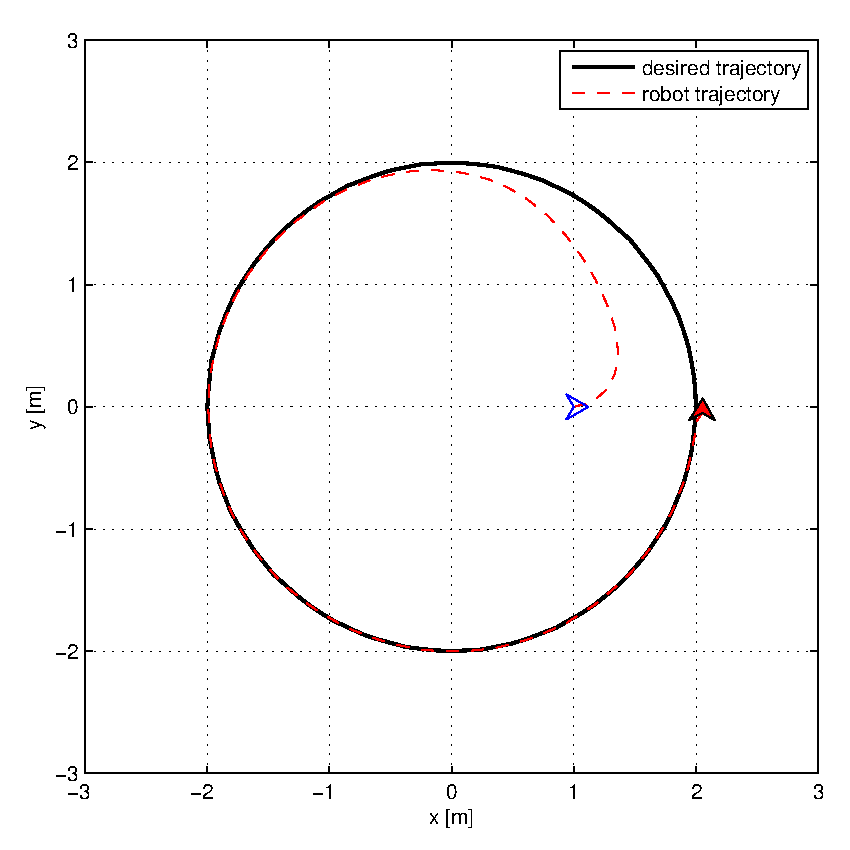
\includegraphics[width=0.48\textwidth,height=0.295\textheight]{circle/trajectory} }
 \subfigure[][]{%
    \label{fig:circle-error}%
    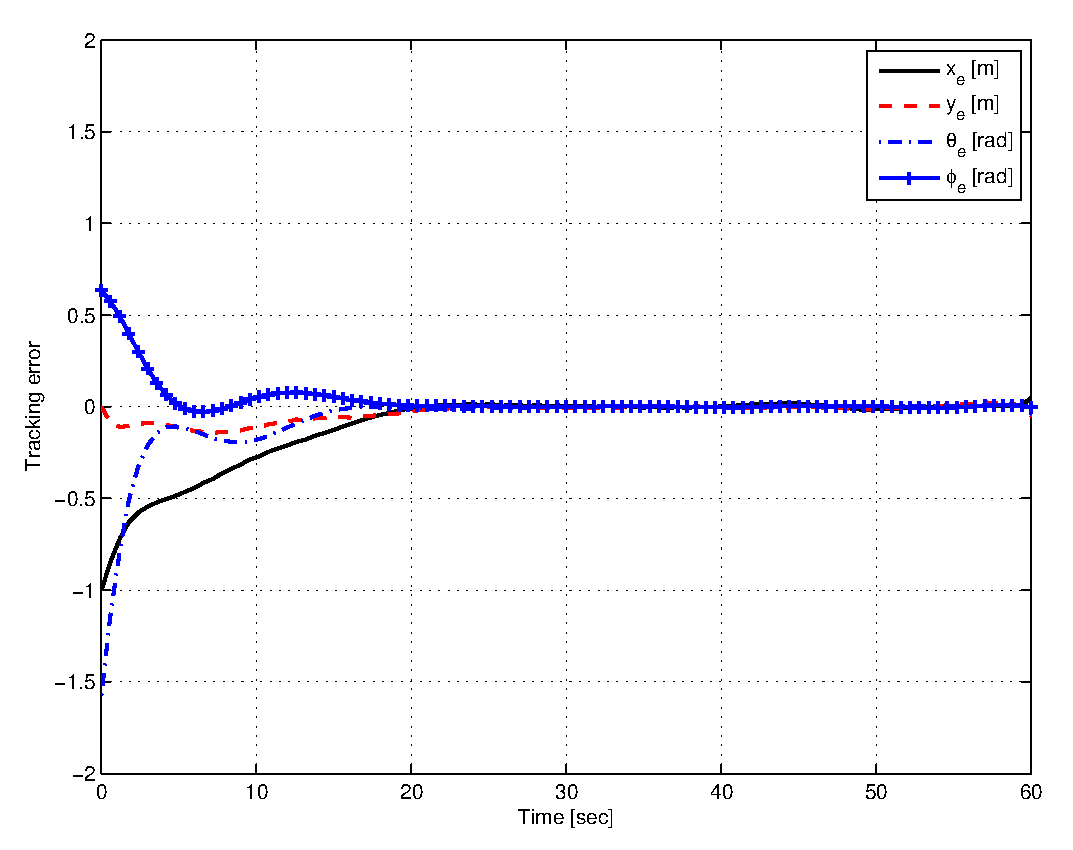
\includegraphics[width=0.48\textwidth,height=0.295\textheight]{circle/error} }
\\
 \subfigure[][]{%
    \label{fig:circle-control-velocity}%
    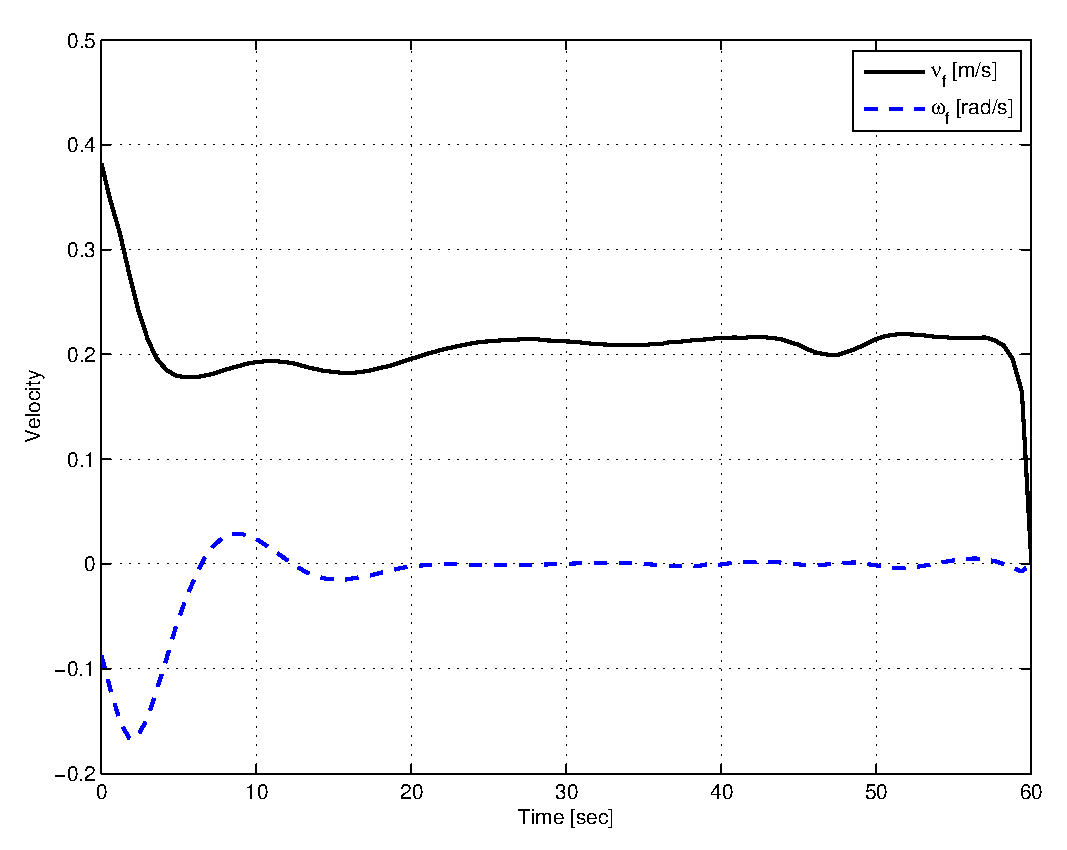
\includegraphics[width=0.48\textwidth,height=0.295\textheight]{circle/control-velocity} }
\subfigure[][]{
  \label{fig:circle-feedback-gain}
    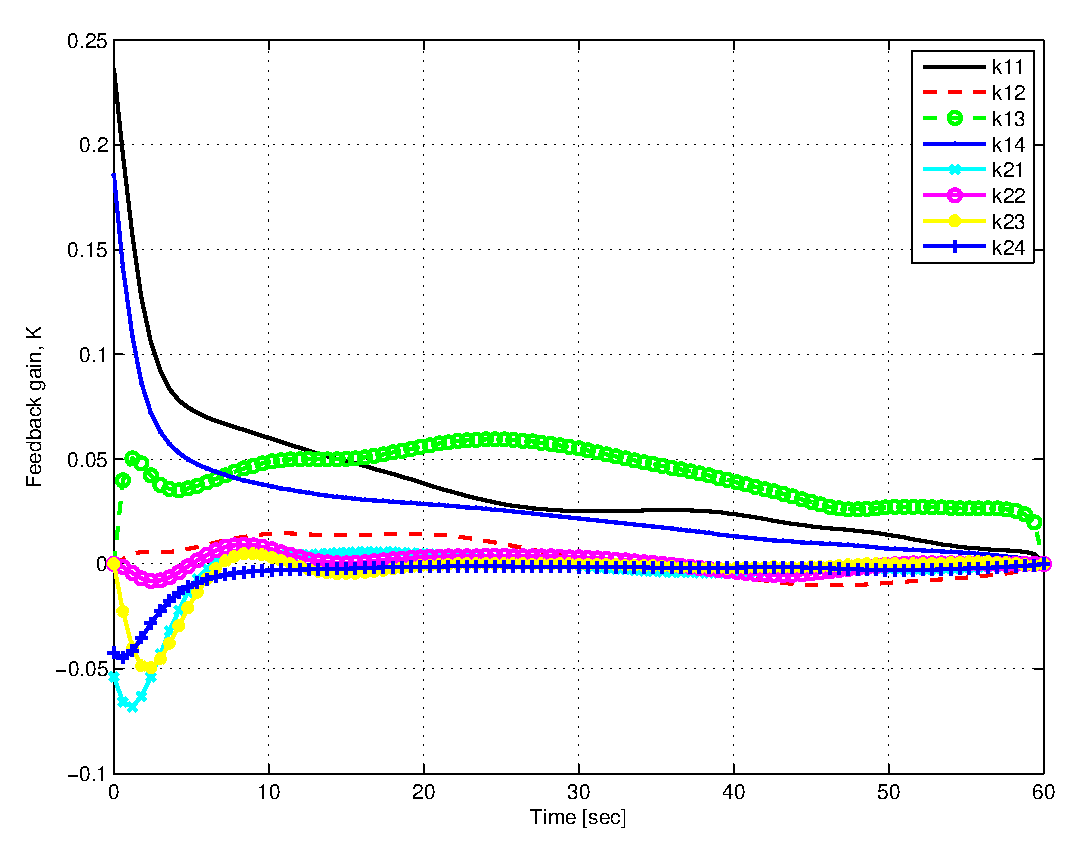
\includegraphics[width=0.48\textwidth,height=0.295\textheight]{circle/feedback-gain}} 
\caption[Performance of circle trajectory.]{Controller's performance in tracking circle trajectory
   \subref{fig:circle-trajectory} trajectory,
   \subref{fig:circle-error} state tracking error, and
    \subref{fig:circle-control-velocity} velocity (control input), and
    \subref{fig:circle-feedback-gain} optimal control law, ${\bf K}^*(t).$
}%
  \label{fig:circle}%
\end{figure}

Hence, the proposed control law ${\bf K}(t),$ is able to provide necessary control actions for the vehicle to track a pre-defined trajectory. It is important to articulate the fact that the proposed universal control law is able to solve trajectory tracking problem of any nonlinear systems of the form~\eqref{eq:systemModel}, but the model~\eqref{eq:modelVehicle} was chosen for the demonstration purpose only. 

 %%%%%%%%%%%%%%%%%%%%
 \section{Summary and Conclusions}
 \label{sec:conclusion}
 We examined a novel universal control law for solving the trajectory tracking problem of a class of nonholonomic systems with drift. Both existence and necessary conditions of optimality for the control law are presented along with their proofs. Numerical results on computing control law and its application in a vehicle with Ackermann steering are presented. As can be seen, vehicle is able to track a predefined trajectory using the proposed control law. It can be shown that this control law is able to solve trajectory tracking problems of other nonholonomic systems, such as unicycle, differential drive mobile robots, and hopping robot in flight-phase. Computation of control law is offline, which is its only drawback and we are currently investing to determine online solution to the proposed universal control law.  It is interesting to note that the system model is not required to be linearized to follow a certain reference trajectory in finite time. However, the proposed control law assumes that the system's state is completely observable, which may be a too restrictive and non realistic hypothesis to model a real-vehicle's control law. Designing partially-observed feedback optimal laws is another possible future research avenue of  this current work. Moreover, the practical realization of this proposed optimal feedback control law on a commercial vehicle is possible as the algorithm can be implemented on a microcontroller due to its computational efficiency.


% \appendices
% \section{Proof of the First Zonklar Equation}
% Some text for the appendix.

% use section* for acknowledgement
%\section*{Acknowledgment}
%
%The authors would like to thank...

\bibliographystyle{IEEEtran}        % Include this if you use bibtex 

\bibliography{bib/refsBooksTRTheses,bib/refsGenericControl,bib/refsSuruzWeb}


\end{document}



